\chapter{Problem pokrycia wierzchołkowego}
%\markboth{Pokrycie wierzchołkowe}{Pokrycie wierzchołkowe}
%\addcontentsline{toc}{chapter}{Pokrycie wierzchołkowe}

\section{Wstęp}
	
Tematem rozdziału będzie przedstawienie problemu minimalnego pokrycia wierzchołkowego. Nieformalnie pokryciem wierzchołkowym nazywamy zbioru wierzchołków, w którym każda krawędź z grafu ma co najmniej jeden koniec. Samo określenie problemu wydaje się być niezwykle proste, jednak rozwiązanie tego problemu jest NP-zupełne. Formalnie problem można zdefiniować następująco.

\section{Przedstawienie problemu}

Problem minimalnego pokrycia wierzchołkowego (VERTEX-COVER) polega na znalezieniu w grafie nieskierowanym $G=(V,E)$ takiego podzbioru  $V' \subseteq V$, że dla każdej krawędzi $\{v,w\} \in E: v \in V' \lor w \in V'$.

\begin{twr}
VERTEX-COVER $\in$ NP-zupełnych.
\end{twr}

\section{Dowód przez redukcje}

\begin{proof}

W pierwszej kolejności należy pokazać, że VERTEX-COVER $\in$ NP. Wejściem dla świadectwa jest graf $G=(V,E)$ oraz podzbiór wierzchołków $V’ \subseteq V$. Zadnie polega na sprawdzeniu, czy każda krawędź ma co najmniej jeden koniec w zbiorze $V’$. Jeśli tak jest, to mamy do czynienia z poprawnym pokryciem wierzchołkowym. Nie trudno zauważyć, że czas potrzebny na to jest liniowy względem liczby krawędzi. Natomiast jeśli graf jest stosunkowo gęsty, to złożoność jest kwadratowa względem liczby wierzchołków. Tak czy inaczej jest wielomianowa w ujęciu rozmiaru danych, co za tym idzie VERTEX-COVER $\in$ NP.

Teraz należy pokazać, że VERTEX-COVER $\in$ NP-trudnych. W tym celu należy skorzystać z redukcji VERTEX-COVER do CLIQUE. Dopełniając graf posiadający klikę otrzymujemy graf, którego pokryciem wierzchołkowym jest wszystko poza kliką. Dopełnienie grafu należy rozumieć jako odwrócenie wszystkich krawędzi. Precyzując, wszystkie krawędzie które należały do grafu $G$ nie należą do grafu dopełnionego $\bar{G}$, a te krawędzie które nie istniały w grafie $G$ istnieje w dopełnionym grafie $\bar{G}$. W dalsze rozważania wykorzystują fakt, że suma krawędzi z grafu $G$ i jego dopełnienia $\bar{G}$ daje graf pełny. Jak również to, że dopełnienie grafu dopełnionego daje graf pierwotny. Wszystko to razem oznacza, że problem maksymalnej kliki jest dualny z problemu minimalnego pokrycia wierzchołkowego. Zatem redukcja opierać się będzie na tezie: graf $G$ zawiera klikę na wierzchołkach $V'$ wtedy i tylko wtedy ,gdy $V-V'$ jest pokryciem wierzchołkowym dopełnionego grafu $\bar{G}$. W celu udowodnienia tej tezy zostanie to rozbite na dwie implikacje.

W pierwszej kolejności zostanie pokazane, że jeśli graf $G$ zawiera klikę na wierzchołkach $V’$, to $V-V’$ jest pokryciem wierzchołkowym dopełnionego grafu $\bar{G}$. Dla wierzchołków $ u,v \in V$ pomiędzy którymi nie istnieje krawędź w $G$ zachodzi, że co najmniej jeden z nich nie należy do kliki, czyli należy do zbioru $V-V’$. Jako, że w grafie dopełnionym $\bar{G}$ pomiędzy wierzchołkami $v$ i $u$ istnieje krawędź to zbiór $V-V’$ pokryje ją. Jako, że krawędź została wybrana w sposób dowolny to rozumowanie jest poprawne dla każdej krawędzi z $\bar{G}$, co kończy dowodzenie pierwszej implikacji.

Teraz pozostało pokazać, że: jeśli $V-V’$ jest pokryciem wierzchołkowym dopełnionego grafu $\bar{G}$ to graf $G$ zawiera klikę na $V’$ wierzchołkach. Zwróćmy uwagę na to że zbiór $V’$ zawiera wszystkie te wierzchołki które nie należą do pokrycia wierzchołkowego, zatem w grafie dopełnionym $\bar{G}$ między nimi nie występuje żadna krawędź. Zachodzi tak ponieważ jeśli którąś parę łączyła by krawędź to co najmniej jeden z tych wierzchołków musiał by należeć  do pokrycia wierzchołkowego. Skoro w grafie dopełnionym $\bar{G}$ między zbiorem tych wierzchołków nie występuje krawędź to w grafie $G$ między wszystkimi tymi wierzchołkami będą występowały krawędzie co z kolei oznacza że na zbiorze $V’$ mamy klikę. To stwierdzenie kończy drugą implikację, ostatecznie wykazując prawdziwość tezy postawionej wcześniej.

Ostatnim krokiem jest określenie złożoności sprowadzenia VERTEX-COVER do CLIQUE. Przy takim postępowaniu należy wpierw stworzyć graf pełny na identycznej liczbie wierzchołków, by później iterując po każdej krawędzi pozostawiać jedynie te krawędzie które nie należały do pierwotnego grafu. Na koniec klika będzie znajdowała się na tych wierzchołkach które nie nie należały do pokrycia wierzchołkowego. Jak widać całość jest złożoności kwadratowej ze względu na ilość wierzchołków, czyli wielomianowa, co kończy cały dowód wykazując że VERTEX-COVER $\in$ NP-zupełny.
\end{proof}

\section{Algorytm aproksymacyjny}

\subsection{Algorytm VERTEX-COVER-DEGREES-APPROX}

	Można odnieść wrażenie że metoda zachłanna będzie przynosiła wyniki bardzo zbliżone do optymalnego, zatem spróbujmy w ten oto sposób podejść do problemu. Możemy wyróżnić dwa sposoby podejścia zachłannego. Pierwszy to taki, który pokrywał by wierzchołki o najwyższym stopniu, idąc za myślą że taki wierzchołek pokryje najwięcej krawędzi zatem naturalnie powinien wchodzić w skład pokrycia wierzchołkowego. Drugie podejście zachłanne to takie, w którym przyglądamy się końca(brzegom) grafu, czyli takim nie izolowanym wierzchołkom, które mają możliwie najmniejszy stopień wierzchołka. Tutaj naturalna jest myśl, że jeśli mamy pokryć te incydentne krawędzie to należało by do pokrycia wybrać wierzchołek z drugiego końca krawędzi. Obie metody w swojej idei wykorzystują najlepsze rozwiązanie lokalne co wydaje się prowadzić do dobrego przybliżenia problemu globalnego. W swoich rozważaniach skupie się na drugim podejściu, dlatego że to pierwsze jest popularnie rozważane w literaturze.
	Oto algorytm realizujący to podejście:

\begin{algorithm}
\caption{VERTEX-COVER-DEGREES-APPROX}\label{euclid}
\begin{algorithmic}[1]
\Function{MyProcedure}{}
\State $C \gets \emptyset$
\State $E' \gets G.E$
\While{$E' \neq \emptyset$} 
\State $\text{weź dowolny nieizolowany wierzchołek }v \newline \text{ o najmniejszym  stoppniu w grafie }G$
\State $\text{weź incydentny wierzchołek }u\text{ z wierzchołkiwm }v \newline \text{ o największym stopniu}$
\State $C \gets C \cup \{u\}$
\State $\text{usuń z } E' \text{ incydentne krawędzie z } u$
\EndWhile
\State \Return C
\EndFunction
\end{algorithmic}
\end{algorithm}


	Rysunek ~\ref{vertex-cover-degrees-approx_example} przedstawia kolejne kroki wykonywania algorytmu VERTEX-COVER-DEGREES-APPROX. W pierwszym kroku wierzchołek o najmniejszym stopniu to 1 a jedyny incydentny z nim wierzchołek który wchodzi do pokrycia to 2. W drugim kroku wierzchołek o najmniejszym stopniu to 7 z nim incydentne są 5 i 6. Oba są tego samego stopnia, zatem do pokrycia wejdzie dowolny z nich w tym przypadku 5. Dalej sytuacja jest klarowna i za pośrednictwem 7 do pokrycia wchodzi 6. Ostatni przebieg to pojedyncza krawędź w rezultacie do pokrycia wchodzi dowolnie wybrany 3. Reasumując pokrycie wierzchołkowe dla tego grafu wynosi 4 (wierzchołki: 2,3,5,6) i jest to optymalne rozwiązanie dla tego grafu.
	
\input{vertex_cover/vertex-cover-degrees-approx_example.tex}	

	Zastanówmy się teraz nad konstrukcją grafu który będzie wpuklał tezę że pokrywanie wierzchołków wyższego stopnia daje gorsze rozwiązanie. Bardzo dobrym przykładem jest graf, który nazwijmy płatkiem śniegu(snowflake). Taki graf składa się z rdzenia i wielu ramion. Poniżej zamieściłem schemat takiego grafu którego rdzeniem jest graf $K_{4}$ i składa się z 4 ramion. Możemy zauważyć że liczbę ramion dla takiego rdzenia może zbiegać do nieskończoności, natomiast liczba wierzchołków incydentnych do rdzenia nie może być więcej niż najniższy stopień wierzchołków do których przylegają. W miarę jak rdzeń grafu jest większy tym można do niego przyłączyć większe ramiona.

\begin{figure}[tbh]
\centering

\begin{tikzpicture}
  \tikzstyle{clique}=[circle,draw=black!75,fill=white!100,minimum size=8mm]
\tikzstyle{covered_node}=[circle,thick,draw=black!75, fill=black!100,minimum size=4mm]
\tikzstyle{uncovered_node}=[circle,thick,draw=black!75, fill=white!20,minimum size=4mm]

  \node [clique,tokens=3] (heart) [label=above left:$K_{4}$] {};
  
  \node [covered_node] (1v1) [above of=heart,xshift=-12mm,yshift=1cm] {}
  	edge node [xshift=5] {4} (heart);
  \node [covered_node] (1v2) [above of=heart,xshift=-4mm,yshift=1cm] {}
  	edge node [xshift=5] {4} (heart);
  \node [covered_node] (1v3) [above of=heart,xshift=4mm,yshift=1cm] {}
  	edge node [xshift=5] {4} (heart);
  \node [covered_node] (1v4) [above of=heart,xshift=12mm,yshift=1cm] {}
  	edge node [xshift=5] {4} (heart);
  \node [uncovered_node] (1v5) [above of=heart,yshift=2cm] {}
  	edge (1v1)
  	edge (1v2)
  	edge (1v3)
  	edge (1v4);
  	
  \node [covered_node] (2v1) [below of=heart,xshift=-12mm,yshift=-1cm] {}
  	edge node [xshift=-5] {4} (heart);
  \node [covered_node] (2v2) [below of=heart,xshift=-4mm,yshift=-1cm] {}
  	edge node [xshift=-5] {4} (heart);
  \node [covered_node] (2v3) [below of=heart,xshift=4mm,yshift=-1cm] {}
  	edge node [xshift=-5] {4} (heart);
  \node [covered_node] (2v4) [below of=heart,xshift=12mm,yshift=-1cm] {}
  	edge node [xshift=-5] {4} (heart);
  \node [uncovered_node] (2v5) [below of=heart,yshift=-2cm] {}
  	edge (2v1)
  	edge (2v2)
  	edge (2v3)
  	edge (2v4);
  	
  \node [covered_node] (3v1) [left of=heart,yshift=-12mm,xshift=-1cm] {}
  	edge node [yshift=-5] {4} (heart);
  \node [covered_node] (3v2) [left of=heart,yshift=-4mm,xshift=-1cm] {}
  	edge node [yshift=-5] {4} (heart);
  \node [covered_node] (3v3) [left of=heart,yshift=4mm,xshift=-1cm] {}
  	edge node [yshift=-5] {4} (heart);
  \node [covered_node] (3v4) [left of=heart,yshift=12mm,xshift=-1cm] {}
  	edge node [yshift=-5] {4} (heart);
  \node [uncovered_node] (3v5) [left of=heart,xshift=-2cm] {}
  	edge (3v1)
  	edge (3v2)
  	edge (3v3)
  	edge (3v4);
  	
  \node [covered_node] (4v1) [right of=heart,yshift=-12mm,xshift=1cm] {}
  	edge node [yshift=5] {4} (heart);
  \node [covered_node] (4v2) [right of=heart,yshift=-4mm,xshift=1cm] {}
  	edge node [yshift=5] {4} (heart);
  \node [covered_node] (4v3) [right of=heart,yshift=4mm,xshift=1cm] {}
  	edge node [yshift=5] {4} (heart);
  \node [covered_node] (4v4) [right of=heart,yshift=12mm,xshift=1cm] {}
  	edge node [yshift=5] {4} (heart);
  \node [uncovered_node] (4v5) [right of=heart,xshift=2cm] {}
  	edge (4v1)
  	edge (4v2)
  	edge (4v3)
  	edge (4v4);

\end{tikzpicture}

\caption{Graf snowflake(4,4)}
\label{vertex-cover-edges-approx_gadget}
%\small
%zakomentarzowany tekst
\end{figure}	
	
	Wierzchołki oznaczone kolorem czarnym zostały nominowane do pokrycia wierzchołkowego grafu plus dodatkowo 3 wierzchołki z $K_{4}$ (nie można mniej dla grafu pełnego). Natomiast można łatwo zauważyć, że jeśli do pokrycia zaliczymy białe wierzchołki plus dodatkowo klikę, to również pokryje nam to graf przy znacznie mniejszej liczbie wierzchołków.
	Oszacujmy współczynnik aproksymacji dla tej rodziny grafów gdzie \textit{k} będzie rozmiarem rdzenia a $m$ liczbą  ramion. Łatwo zauważyć że przypadek pesymistyczny to taki gdzie liczbę i rozmiar ramion będziemy maksymalizowali, natomiast rozmiar rdzenia będziemy minimalizowali. Aby własność doboru nieodpowiednich wierzchołków była zachowana to liczba wierzchołków połączonych z rdzeniem musi być nie większa od rozmiaru rdzenia.  Minimalny graf o jak największej liczbie krawędzi to graf pełny.
	 W skład pokrycia optymalnego będzie wchodził zawsze cały rdzeń grafu, czyli $k$ wierzchołków a dodatkowo $m$ wierzchołków z każdego ramienia po tym wierzchołku który nie jest połączony z rdzeniem. W przypadku rozwiązania proponowanego przez algorytm mamy $k-1$ wierzchołków z rdzenia oraz $m*k$ wierzchołków ze wszsytkich ramion. W rezultacie otrzymujemy: $\frac{C}{C^{*}} = \frac{k-1 + m*k}{k+m} \le m*k$. Zatem zależność jest liniowa co świadczy o słabym współczynniku aproksymacji.

\subsection{Algorytm VERTEX-COVER-EDGES-APPROX}

	 Przyjrzyjmy się teraz innemu podejściu do problemu. Proponowane rozwiązanie to wybrać losową krawędź, dwa jej końce dodać do pokrycia wierzchołkowego, po czym usunąć wszsytkie incydętne z nimi krawędzie. Oto algorytm realizujący to podejście:

\begin{algorithm}
\caption{VERTEX-COVER-EDGES-APPROX}\label{euclid}
\begin{algorithmic}[1]
\Function{MyProcedure}{}
\State $C \gets \emptyset$
\State $E' \gets G.E$
\While{$E' \neq \emptyset$} 
\State $\text{weź dowolna krawędź}(u,v) \in E'$
\State $C \gets C \cup \{u,v\}$
\State $\text{usuń z } E' \text{ incydentne krawędzie z } u \text{ lub } v $
\EndWhile
\State \Return C
\EndFunction
\end{algorithmic}
\end{algorithm}


	Teraz wykonajmy ten sam algorytm dla poprzedniego grafu. W pierwszym kroku w dowolny sposób wybraliśmy krawędź \{1,2\}, dodaliśmy te wierzchołki do pokrycia i usuneliśmy wszsytkie incydętne krawędzie. W drugim kroku analogicznie została wybrana dowolna krawędź \{5,7\}, wierzchołki dodane do pokrycia, a następnie usunięte wszystkie incydentne krawędzie. Całe rozumowanie jest powtarzane aż w rezulatcie do pokrycia wierzchołkowego zostały przypisane wierzchołki: 1,2,3,4,5,7.

\begin{figure}[tbh]
\centering

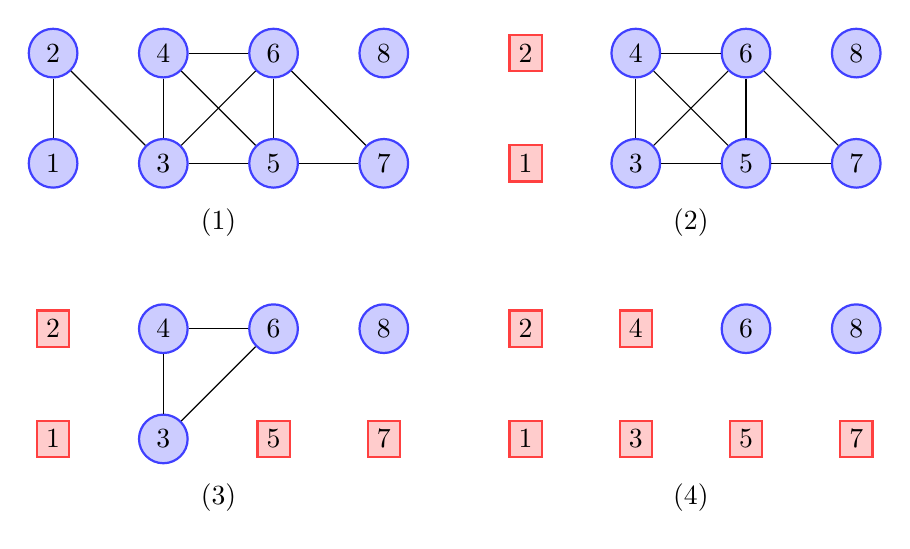
\begin{tikzpicture} [node distance=1.4cm]

\tikzstyle{unmark_vertex}=[circle,thick,draw=blue!75,fill=blue!20,minimum size=5mm]
\tikzstyle{mark_vertex}=[rectangle,thick,draw=red!75,
  			  fill=red!20,minimum size=4mm]

  \begin{scope}
  	\node [unmark_vertex] (v1) {1};
  	\node [unmark_vertex] (v2) [above of=v1] {2}
  		edge (v1);
  	\node [unmark_vertex] (v3) [right of=v1] {3}
  		edge (v2);
  	\node [unmark_vertex] (v4) [right of=v2] {4}
  		edge (v3);
  	\node [unmark_vertex] (v5) [right of=v3] {5}
  		edge (v3)
  		edge (v4);
  	\node [unmark_vertex] (v6) [right of=v4] {6}
  		edge (v3)
  		edge (v4)
  		edge (v5);
  	\node [unmark_vertex] (v7) [right of=v5] {7}
  		edge (v5)
  		edge (v6);
  	\node [unmark_vertex] (v8) [right of=v6] {8};

	\node at (2.1cm, -0.75cm) {\text{(1)}};
  \end{scope}
  
  \begin{scope}[xshift=6cm]
  	\node [mark_vertex] (v1) {1};
  	\node [mark_vertex] (v2) [above of=v1] {2};
  	\node [unmark_vertex] (v3) [right of=v1] {3};
  	\node [unmark_vertex] (v4) [right of=v2] {4}
  		edge (v3);
  	\node [unmark_vertex] (v5) [right of=v3] {5}
  		edge (v3)
  		edge (v4);
  	\node [unmark_vertex] (v6) [right of=v4] {6}
  		edge (v3)
  		edge (v4)
  		edge (v5);
  	\node [unmark_vertex] (v7) [right of=v5] {7}
  		edge (v5)
  		edge (v6);
  	\node [unmark_vertex] (v8) [right of=v6] {8};

	\node at (2.1cm, -0.75cm) {\text{(2)}};
  \end{scope}
  
  \begin{scope}[yshift=-3.5cm]
  	\node [mark_vertex] (v1) {1};
  	\node [mark_vertex] (v2) [above of=v1] {2};
  	\node [unmark_vertex] (v3) [right of=v1] {3};
  	\node [unmark_vertex] (v4) [right of=v2] {4}
  		edge (v3);
  	\node [mark_vertex] (v5) [right of=v3] {5};
  	\node [unmark_vertex] (v6) [right of=v4] {6}
  		edge (v3)
  		edge (v4);
  	\node [mark_vertex] (v7) [right of=v5] {7};
  	\node [unmark_vertex] (v8) [right of=v6] {8};

	\node at (2.1cm, -0.75cm) {\text{(3)}};
  \end{scope}
  
  \begin{scope}[yshift=-3.5cm, xshift=6cm]
  	\node [mark_vertex] (v1) {1};
  	\node [mark_vertex] (v2) [above of=v1] {2};
  	\node [mark_vertex] (v3) [right of=v1] {3};
  	\node [mark_vertex] (v4) [right of=v2] {4};
  	\node [mark_vertex] (v5) [right of=v3] {5};
  	\node [unmark_vertex] (v6) [right of=v4] {6};
  	\node [mark_vertex] (v7) [right of=v5] {7};
  	\node [unmark_vertex] (v8) [right of=v6] {8};

	\node at (2.1cm, -0.75cm) {\text{(4)}};
  \end{scope}
\end{tikzpicture}

\caption{Przykład wykonania algorytmu VERTEX-COVER-EDGES-APPROX}
\label{vertex-cover-edges-approx_example}
%\small
%zakomentarzowany tekst
\end{figure}

Porównując te dwa podejścia można odnieść wrażenie, że ostatni algorytm nie jest godny uwagi, lecz spróbójmy określić współczynnik aproksymacji dla algorytmu VERTEX-COVER-EDGES-APPROX.

\begin{twr}
VERTEX-COVER-DEGREES-APPROX jest 2 aproksymowalne [do po polsku]
\end{twr}

\begin{proof}
W pierwszej kolejności pokażmy że zbiór z wyjścia algorytmu VERTEX-COVER-EDGES-APPROX jest rzeczywiście pokryciem wierzchołkowym. Pętla z 4. linii wykonuje się do momentu aż wszystkie krawędzie nie zostaną pokryte. Wewnątrz w linii 5. do pokrycia dodajemy oba końce losowo wybranej krawędzi, następnie usuwając te krawędzie, które pokryte są przez dodane wierzchołki. W rezultacie zostają jedynie usunięte te krawędzie które są pokryte, a do zbioru wyjściowego wchodzą te wierzchołki przy których krawędź jeszcze nie została pokryta. W tym procesie otrzymany zbiór wierzchołków jest prawidłowym pokryciem wierzchołkowym dla zadanego grafu.

Przyjrzyjmy się teraz jakości tego rozwiązania. Algorytm VERTEX-COVER-EDGES-APPROX w linii 5. dodaje dwa wierzchołki z jednej krawędzi do pokrycia wierzchołkowego. W linii 7. zostają usunięte wszystkie incydentne krawędzie w rezultacie. Tak postępując można zaobserwować, że żadne losowo wybrane krawędzie nie mają wspólnego wierzchołka. Zatem zbiór zawiera tyle wierzchołków ile wynosi podwojona liczba losowych krawędzi. Zauważmy, że pokrycie optymalne musi analogicznie pokryć wszystkie krawędzie, w tym również te, które losowo wybraliśmy. W rezultacie pokrycie generowane przez algorytm VERTEX-COVER-EDGES-APPROX jest nie więcej niż 2 krotnie większe od optymalnego.
\end{proof}

Choć algorytm VERTEX-COVER-EDGES-APPROX posiada znacząco niższy współczynnik aproksymacji od algorytmu VERTEX-COVER-DEGREES-APPROX to widać, że swoją przewagę zawdzięcza jedynie szczególnym przypadkom. W ogólności algorytm VERTEX-COVER-EDGES-APPROX będzie zwracał gorsze rozwiązanie od algorytmu VERTEX-COVER-DEGREES-APPROX.